\documentclass{article}
\usepackage[final,nonatbib]{neurips_2019}
\usepackage[utf8]{inputenc}
\usepackage[T1]{fontenc}
\usepackage{hyperref}
\usepackage{url}
\usepackage{booktabs}
\usepackage{graphicx}
\usepackage{amsmath}
\usepackage{microtype}
\usepackage{enumitem}
\usepackage{pifont}
\usepackage{xcolor}
\newcommand{\Spade}{\ding{171}}
\newcommand{\Club}{\ding{168}}
\newcommand{\Heart}{\textcolor{red!75!black}{\ding{170}}}
\newcommand{\Diam}{\textcolor{red!75!black}{\ding{169}}}
\newcommand{\file}[1]{{\small\texttt{#1}}}
\makeatletter\renewcommand{\@notice}{}\makeatother % no conference footer
\setlist{itemsep=1pt,topsep=2pt}

\title{Reading the Order Flow: Information Extraction and Leakage\\in Learned Agents for the Trading Game Figgie\\[4pt]\large Midterm report}

\author{%
  Nicholas Erup Larsen \\
  IIIS, Tsinghua University \\
  \texttt{nglsls26@mails.tsinghua.edu.cn} \\
  Student ID: 2026400695 \\
  \And
  Adriaan Van der Berg \\
  IIIS, Tsinghua University \\
  \texttt{adla26@mails.tsinghua.edu.cn} \\
  Student ID: 2026403362 \\
}

\begin{document}
\maketitle

\begin{abstract}
Figgie is a four-player card-trading game whose scoring (goal) suit is hidden.
Every published Figgie agent infers the goal suit from its own cards, yet every public trade also carries information about what the trader holds.
Our project asks how much the order flow reveals, whether reinforcement-learning (RL) agents with memory learn to read it, and whether agents that leak their own hand are easier to exploit.
At the midterm we have a shared game engine with 25 agents ported from four public sources (two of them ported decision for decision), a reproduction of the only RL agent for Figgie that matches or beats its reported numbers, and a 16{,}000-game tournament of 29 agents.
A simple model of the public trades raises goal-suit accuracy from 39\% (own hand only) to 54\% by the end of a game.
A first linear probe of the PPO agent's recurrent state finds that its memory holds no more about the goal suit than the card-counting posterior it is given as input (41\% against 43\%), although the input itself supports 65\%.
\end{abstract}

\section{Problem and questions}
In Figgie, 40 cards are dealt from one of 12 equally likely decks: one suit has 12 cards, one has 8 and two have 10.
The goal suit is the same-colour partner of the 12-card suit (\Spade$\leftrightarrow$\Club, \Heart$\leftrightarrow$\Diam), so it has 8 or 10 cards.
Each of the four players antes \$50 into a \$200 pot. At the end each goal card pays its holder \$10 and the rest of the pot goes to whoever holds the most goal cards.
Players trade continuously by quoting bids and asks in each suit, and every trade is public.
Because goal cards pay out, players pay more for the suit they believe is the goal, so a player who eagerly buys \Club{} probably holds many clubs and believes \Club{} is the goal.

Existing agents, such as figment's Bayesian market maker~\cite{figment}, Figgie-bot's exact inference~\cite{figgiebot} and the CS224R PPO agent~\cite{cs224r}, compute the goal-suit posterior from their own cards and at most a count of cards seen changing hands. None of them models \emph{why} an opponent trades.
Figgie is a clean test of a general question in partially observed multi-agent RL: does an agent trained only on reward learn to infer hidden state from other agents' behaviour?
The hidden state is tiny (12 decks), so the exact belief is cheap to compute and can be compared with what the network represents.
The approved proposal asks three questions:
\begin{enumerate}[label=Q\arabic*.]
  \item Revelation. How much does the public trade history reveal about the goal suit beyond a player's own hand, and how quickly? We measure the gap $\Delta_{\text{rev}}(t)$ in bits of goal-suit log-loss.
  \item Extraction. Do PPO agents with memory (none $<$ minGRU $<$ GRU $<$ transformer) learn to infer the goal suit, as tested by probing, attribution and causal interventions on their hidden state?
  \item Leakage and exploitability. Does an agent's leakage $L_a$ (how well its actions predict its hand) correlate with its exploitability $\hat\varepsilon_a$, measured by a learned PPO best response?
\end{enumerate}

\section{Work completed}

\subsection{A shared engine and verified agents}
All data is simulated in our engine (\file{figgie/engine.py}), which implements the standard rules and the CS224R discretisation: 240 ticks, one action per player per tick in a random order, 257 discrete actions, prices \$1--\$30, and every trade wipes the book.
The simulator logs the deck and all hands, so every sample carries exact ground truth.
One game takes about 11\,ms on one CPU core (85{,}000 decisions/s).
We ported 25 agents from four public sources (Table~\ref{tab:ports}).
For figment and Figgie-bot we ran the original code inside its own simulator and fed the same observations to our port. Every decision was identical (144{,}000 of 144{,}000 and 64{,}000 of 64{,}000), and so was every goal posterior (\file{results/verify\_ports.json}).
The figgie-auto bots run in real time with wall-clock sleeps and an entropy-seeded RNG, so they cannot be replayed and were only checked by code review.

\begin{table}[h]
  \centering\small
  \caption{Ported sources and how each port was checked (\file{RESULTS.md} \S1, \file{results/verify\_ports.json}).}
  \label{tab:ports}
  \begin{tabular}{@{}lll@{}}
    \toprule
    Source & How the port was checked & Result \\
    \midrule
    CS224R report~\cite{cs224r} (5 baselines, PPO) & reimplemented from the text & numbers reproduced (\S2.2) \\
    figment~\cite{figment} (5 agents) & decisions of 3 agents vs.\ original & 144{,}000 / 144{,}000 identical \\
    Figgie-bot~\cite{figgiebot} (8 agents) & decisions of 4 agents vs.\ original & 64{,}000 / 64{,}000 identical \\
    figgie-auto~\cite{figgieauto} (7 bots) & code review only & not replayable \\
    \bottomrule
  \end{tabular}
\end{table}

\subsection{Reproducing the CS224R PPO agent}
The CS224R agent~\cite{cs224r} is the only RL agent for Figgie and released no code, so we reimplemented it from the report.
A 69-dimensional observation (own hand, cash, all quotes, tick, a card-counting goal posterior and expected card values) feeds a two-layer MLP, a 128-unit GRU cell and a masked categorical actor over the 257 actions (\file{figgie/rl/policy.py}).
Training is behaviour cloning from the Bayesian baseline followed by recurrent PPO with potential-based reward shaping and prioritised fictitious self-play, using 32 environments $\times$ 512 steps per update.
Version v1 clones all actions equally. Version v2 up-weights lift actions 15$\times$ in cloning and adds a lift bonus in PPO.
Every detail the report omits was filled with a documented guess (\file{DESIGN.md}).
Table~\ref{tab:cs224r} shows the matchups the report uses for its headline claims. PPO-v2 after 300 updates (4.9\,M steps) matches or beats every reported number, including about half the games won against the strongest heuristic-only table (52\% against 54\% reported).
Our agents earn about twice the reported profit at tables with the Random baseline. Our Random samples uniformly from the legal actions, including \$30 bids, and loses about \$200 per game, whereas the report does not define its Random.
Without behaviour cloning, PPO beats Random but loses to strong tables.
Each configuration was trained with one seed only.

\begin{table}[h]
  \centering\small
  \caption{CS224R Table~1 matchups, 1000 games each, seats rotated, greedy actions. Profit in \$/game (95\% CI about $\pm$4--5) and win rate (\file{RESULTS.md} \S2, \file{results/cs224r\_eval.json}). FV = FairValue, R = Random, Cons = Conservative, MM = MarketMaker.}
  \label{tab:cs224r}
  \begin{tabular}{@{}lrrrrr@{}}
    \toprule
    Opponents & Reported v1 & Ours v1 & Reported v2 & Ours v2 & Ours, no BC \\
    \midrule
    3$\times$Random & +118, 89\% & +135, 76\% & +164, 98\% & +278, 99\% & +178, 95\% \\
    Bayes + 2$\times$R & +77, 4\% & +107, 38\% & +112, 10\% & +233, 92\% & +144, 64\% \\
    FV + Cons + MM & +6, 33\% & +2, 28\% & +8, 54\% & +21.5, 52\% & +0.2, 30\% \\
    FV + Bayes + MM & +2, 22\% & $-$6, 19\% & +2, 36\% & +12.7, 53\% & $-$17, 20\% \\
    \bottomrule
  \end{tabular}
\end{table}

\subsection{A 29-agent tournament}
To rank agents from different sources on equal terms we ran a duplicate tournament (\file{scripts/tournament.py}).
Each of 4000 tables draws four distinct agents and plays one deal under all four seat rotations, giving 16{,}000 games.
We report mean profit with table-clustered 95\% CIs, win rate, pairwise Elo and TrueSkill.
The field includes three controls: uniform random play, a no-information market maker that values every card at \$8.8 (ConstVal), and PotMM with its suit labels scrambled each game (PotValShuffled).
The uniform-random agents lose so much that sitting next to them dominates the ranking, so Table~\ref{tab:tour} uses a second run (another 16{,}000 games) with the other 26 agents.
No agent dominates. Four agents from three sources are statistically tied at +15 to +22 \$/game, and profit, win rate and Elo each name a different winner.
The no-information control sits mid-table at +2.6, which shows that price levels without any belief explain the agents around it, and scrambling the goal suit makes PotMM the worst agent at $-$48.4, so goal-suit information is worth a great deal.
PPO-v2 has the highest win rate and Elo even though it was trained only against the five CS224R baselines and its own snapshots.

\begin{table}[h]
  \centering\small
  \caption{Selected rows of the 26-agent tournament without uniform-random agents, about 2400 games per agent (\file{results/tournament\_norandom.md}). Full table in \file{RESULTS.md} \S3.}
  \label{tab:tour}
  \begin{tabular}{@{}rllrrr@{}}
    \toprule
    Rank & Agent & Source & Profit \$/game & Win rate & Elo \\
    \midrule
    1 & AdaptiveMM & figment & +22.2 $\pm$ 2.4 & 31.7\% & 1565 \\
    2 & BayesianMM & figment & +18.4 $\pm$ 2.3 & 28.5\% & 1566 \\
    3 & Bayesian & CS224R & +16.1 $\pm$ 2.6 & 42.0\% & 1551 \\
    4 & PPO-v2 & CS224R (ours) & +15.5 $\pm$ 2.2 & 44.7\% & 1574 \\
    7 & PotMM & Figgie-bot & +11.4 $\pm$ 2.3 & 43.4\% & 1552 \\
    14 & ConstVal (no-info control) & Figgie-bot & +2.6 $\pm$ 3.0 & 38.2\% & 1510 \\
    19 & PPO, no BC & CS224R (ours) & $-$3.5 $\pm$ 2.1 & 18.3\% & 1469 \\
    26 & PotValShuffled (scrambled control) & Figgie-bot & $-$48.4 $\pm$ 3.6 & 15.9\% & 1345 \\
    \bottomrule
  \end{tabular}
\end{table}

\begin{figure}[t]
  \centering
  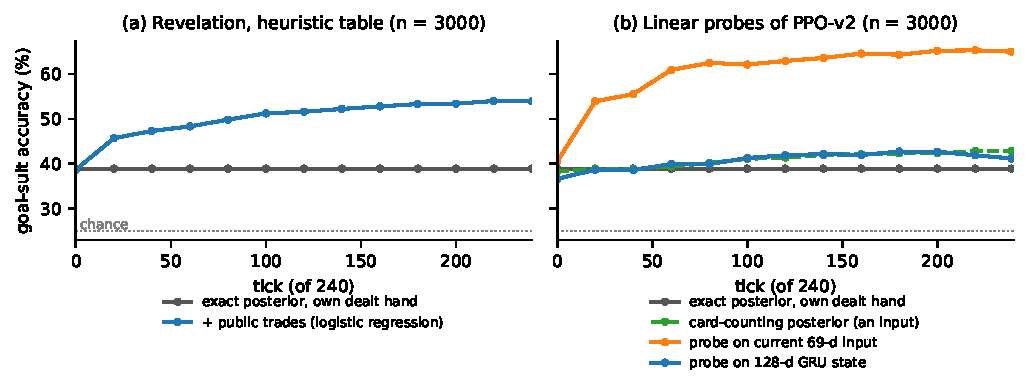
\includegraphics[width=\textwidth]{midterm_results.pdf}
  \caption{Goal-suit accuracy over the game for the player at seat 0, 3000 games each, 5-fold cross-validated. (a)~Q1: the seat-0 BayesianMM against Bayesian, PotMM and Fundamental. A logistic regression on the exact hand-only posterior plus summary features of the public trades beats the hand-only posterior from the first trades on (\file{results/proposal\_revelation.json}). (b)~Q2: PPO-v2 replaces BayesianMM at seat 0. Linear probes read the goal suit from the agent's current input or from its GRU state (\file{results/probe\_ppo\_v2.json}). Chance is 25\%.}
  \label{fig:results}
\end{figure}

\subsection{Q1: the public trades reveal the goal suit}
As a first measurement of revelation we simulated 3000 games at one fixed table (figment's BayesianMM at seat 0 against Bayesian, PotMM and Fundamental) and, at every 20 ticks, predicted the goal suit for seat 0 in two ways (\file{scripts/proposal\_figure.py}).
The baseline is the exact Bayesian posterior given only seat 0's dealt hand.
The order-flow model is a logistic regression that adds simple features of the public trades so far: each opponent's net purchases per suit, the largest net position per suit, the number of trades per suit and their mean price.
Figure~\ref{fig:results}a shows that the trades help from the first 20 ticks and keep helping all game.
By tick 240 accuracy rises from 38.9\% to 54.0\% and log-loss falls from 1.88 to 1.54 bits, so $\Delta_{\text{rev}}(240)\approx 0.35$ bits (\file{results/proposal\_revelation.json}, $n=3000$).
This is a lower bound on revelation, since a linear model on hand-crafted summaries throws away the order and timing of trades and the quotes that did not trade.
The proposed sequence model should raise it.

\subsection{Q2: a first linear probe of PPO-v2}
The midterm milestone in the proposal was a first probe of the PPO agent.
We replaced BayesianMM at seat 0 by PPO-v2 (against Bayesian, PotMM and Fundamental) for 3000 games and recorded its 69-dimensional input and its 128-dimensional GRU state at every 20 ticks (\file{scripts/probe\_ppo.py}, about 10 minutes on a laptop CPU).
At each tick we fit 5-fold cross-validated logistic regressions on standardised features that predict the true goal suit~\cite{probes}.
The actor reads only the GRU state, so whatever goal-suit belief drives the agent's trades must pass through it.

Figure~\ref{fig:results}b and Table~\ref{tab:probe} show a clear negative result for this agent.
The GRU state is no more informative than the card-counting posterior that is one of the agent's inputs: 41.2\% accuracy at the last tick against 42.9\%.
Yet a linear probe on the current input alone reaches 65.0\% and 1.27 bits, so the information is available to the agent at every step and it does not keep it in a linearly readable form.
That is consistent with how PPO-v2 was trained, by cloning a baseline whose belief uses only card counts and then optimising profit against such baselines.
The input probe is also a second, stronger lower bound for Q1 at this table: everything in the input is observable by seat 0, and it already beats the hand-only posterior by 0.61 bits.
Two caveats apply. A linear probe can miss a nonlinear code, so the next step adds small MLP probes, and the card-counting posterior is badly calibrated (1.98 bits, worse than the 1.88 of the hand-only posterior although slightly more accurate), so it is a weak reference for log-loss.
Concatenating input and GRU state (62.8\%) does slightly worse than the input alone, a sign that the probes are close to over-fitting with 2400 training games and need tuned regularisation.

\begin{table}[h]
  \centering\small
  \caption{Goal-suit accuracy and log-loss (bits) for PPO-v2 at seat 0, 3000 games, 5-fold CV (\file{results/probe\_ppo\_v2.json}).}
  \label{tab:probe}
  \begin{tabular}{@{}lrrrr@{}}
    \toprule
    Predictor & Acc., tick 100 & Acc., tick 239 & Bits, tick 100 & Bits, tick 239 \\
    \midrule
    Exact posterior, own dealt hand & 38.9\% & 38.9\% & 1.88 & 1.88 \\
    Card-counting posterior (input features) & 41.1\% & 42.9\% & 2.02 & 1.98 \\
    Linear probe, GRU state & 41.3\% & 41.2\% & 1.96 & 1.94 \\
    Linear probe, current input & 62.1\% & 65.0\% & 1.35 & 1.27 \\
    \bottomrule
  \end{tabular}
\end{table}

\section{Remaining plan}
The engine is CPU-bound, so most of the cost is rollouts, and all runs fit on a two-GPU server we already have access to (about 80 hours in total, no rented compute).
\begin{itemize}
  \item Memory agents (16--29 Nov). PPO policies with no memory, a minGRU, a GRU and a transformer over the trade history, 3 seeds each (12 runs of about 50\,M steps). The supervised sequence model for Q1, trained on the full trade history and on several opponent populations.
  \item Interpretability (30 Nov--13 Dec). Linear and MLP probes of every agent against the true goal suit and the hand-only posterior, giving an extraction score $E_a$ from 0 (hand only) to 1 (as good as the Q1 model). Attribution of beliefs to past trades, steering along the probe direction~\cite{actadd}, activation patching between matched games, and ablation to price the belief in \$/game.
  \item Leakage and exploitability (7--20 Dec). A classifier per agent that predicts the agent's hand from its own actions, giving $L_a$ in bits over the prior. One PPO best response per agent (about 10 agents $\times$ 20\,M steps) against three copies of it, minus a no-information control, giving $\hat\varepsilon_a$, and the rank correlation of $L_a$ with $\hat\varepsilon_a$.
  \item Poster for the week-15 session (21--27 Dec) and the final NeurIPS-format report with a cleaned repository and one reproduction script (by 8 Jan).
\end{itemize}
The central tests stay those of the proposal: whether RL agents read the trades ($E_a>0$), whether better memory helps, and whether leakier agents lose more to a best response.

\section{Caveats}
\begin{itemize}
  \item Every PPO number so far comes from a single seed. The memory agents will use three seeds each, and we will rerun PPO-v2 with more seeds before comparing it with them.
  \item The CS224R report leaves many details open (observation layout, Random's behaviour, several PPO hyperparameters). Our guesses are listed in \file{DESIGN.md} and change absolute profits, though not the ranking.
  \item Tournament numbers depend on the field and are not an equilibrium analysis. Exploitability has no closed form in four-player general-sum games, which is why Q3 uses learned best responses~\cite{timbers}.
  \item The Q1 result covers one table of heuristic agents. Revelation depends on who is trading, so the final measurement will be repeated per opponent population.
\end{itemize}

{\small
\begin{thebibliography}{99}\setlength{\itemsep}{0pt}\setlength{\parskip}{0pt}
\bibitem{figment} mneha05. \newblock figment: a self-play market-making arena for Figgie-style card markets. \newblock \url{https://github.com/mneha05/figment}.
\bibitem{figgiebot} revilo-25. \newblock Figgie-bot. \newblock \url{https://github.com/revilo-25/Figgie-bot}.
\bibitem{figgieauto} 0xDub. \newblock figgie-auto. \newblock \url{https://github.com/0xDub/figgie-auto}.
\bibitem{cs224r} D.~Li Yang. \newblock Reinforcement learning for Figgie: learning negotiation as a first-class skill. \newblock Stanford CS224R project report, 2026.
\bibitem{timbers} F.~Timbers et al. \newblock Approximate exploitability: learning a best response. \newblock In \emph{IJCAI}, 2022.
\bibitem{actadd} A.~M.~Turner et al. \newblock Steering language models with activation engineering. \newblock arXiv:2308.10248, 2023.
\bibitem{probes} G.~Alain and Y.~Bengio. \newblock Understanding intermediate layers using linear classifier probes. \newblock arXiv:1610.01644, 2016.
\end{thebibliography}
}

\end{document}
